\section{Nonlinear Multilayer Perceptron Heads}
\label{sec:mlp}

\subsection{Purpose and comparison design}

This section tests whether a compact nonlinear multilayer perceptron (MLP)
improves prediction when it receives the same clinical variables as the models
in Section~\ref{sec:benchmark}.  The diagnostic MLP is compared with logistic
regression, XGBoost and 3 pretrained tabular foundation models (TFMs).  The
prognostic MLP is compared with Cox regression, a random survival forest (RSF),
the TabPFN landmark approach and SurvivalPFN.  These comparisons address the
main question: does adding a trainable nonlinear head improve on the conventional
and foundation-model results already obtained from the clinical data?

\noindent\textbf{Data used in this section.} The main MLP comparison uses the
same processed real SEER cohorts, 17 clinical predictors and held-out evaluation
partitions as Section~\ref{sec:benchmark}: 2,672 patients for diagnosis and 462
for prognosis. A separate exploratory analysis uses the fixed TabPFN embedding
datasets from Section~\ref{sec:transformations}, with 512 diagnostic coordinates
and 1,024 prognostic coordinates for those same patients. No synthetic records
or Erlangen patients are used. Section~\ref{sec:benchmark} compared conventional
and pretrained model families; this section adds a trainable MLP and asks whether
its nonlinear prediction head improves on those existing results.

Only observed patient records are used for training in the main clinical
comparison.  Diagnosis
is evaluated on the same 5 repeats of 5-fold cross-validation among 2,672
patients, and prognosis on the same 5 predefined 70/30 splits among 462 patients.
All preprocessing and model fitting are confined to the training portion of
each fold or split, and performance is measured on the held-out real patients.
The synthetic augmentation experiment is presented separately in
Section~\ref{sec:augmentation}.

A secondary analysis applies an MLP to previously computed TabPFN
representations.  It asks whether a nonlinear head performs better than a
regularized logistic or Cox head when both receive the same representation.  It
does not compare clinical variables with representations.  Because the TabPFN
representations were produced from the complete cohort before the evaluation
partitions were formed, this analysis cannot provide a fully isolated
train--test comparison and is treated as exploratory.

Three predefined network initializations were evaluated for every MLP.  This
produced 75 diagnostic and 15 prognostic fits for each input type, or 180 MLP
evaluation fits in total.  A separate training-stage fit selected the number of
epochs for each task, evaluation partition, input type and initialization.

\subsection{Network architecture and task-specific outputs}
\label{sec:mlp:architecture}

Both MLPs are small feed-forward networks rather than additional foundation
models.  Each hidden layer uses a linear transformation, a rectified linear
unit (ReLU) activation and 20\% dropout.  Batch normalization is not used.  The
networks are optimized with Adam with decoupled weight decay (AdamW), using a
learning rate of $10^{-3}$ and weight decay of $10^{-4}$.  These settings were
specified before the matched evaluation and were not chosen by comparing
performance on the held-out patients.

The diagnostic network returns one logit, which is converted to a probability
of liver metastasis, and is trained with binary cross-entropy.  Class weighting
is not used.  The prognostic network follows the neural Cox formulation of
\citet{Katzman2018}: it returns one log-relative-risk value and minimizes the
negative Cox partial log-likelihood.  Tied event times use the Breslow
approximation.  After fitting, a Breslow baseline cumulative hazard is estimated
from the same training patients so that survival probabilities can be obtained
at 12, 24 and 36 months.  Full-batch optimization is used for prognosis so that
each Cox risk set contains all relevant training patients.

\begin{table}[htbp]
\centering\scriptsize
\setlength{\tabcolsep}{2.5pt}
\caption{MLP architecture used in the matched evaluation.  Input widths are
those obtained after training-only preprocessing.  The prognostic clinical
width varies between 26 and 27 because retained categories and constant columns
can differ across training splits.}
\label{tab:mlp:architecture}
\begin{tabularx}{\linewidth}{@{}p{1.3cm}p{2.45cm}p{1.15cm}p{1.75cm}Yp{1.85cm}p{1.15cm}@{}}
\toprule
Task & Inputs after preprocessing & Hidden widths & Activation / dropout & Output & Training objective & Batch \\
\midrule
\csname @@input\endcsname{tables/mlp_heads/architecture_rows.tex}
\bottomrule
\end{tabularx}
\end{table}

For the clinical MLPs, rare categorical levels are pooled, categories are
one-hot encoded, continuous variables are standardized and constant columns are
removed.  Every one of these steps is estimated anew from the corresponding
training patients.  This produces 31 diagnostic columns and 26 or 27 prognostic
columns.  The exploratory representation analysis uses 512 diagnostic and
1,024 prognostic inputs; their means and standard deviations are also estimated
from the relevant training partition.  Patient identifiers, outcomes,
follow-up times and variables defining the evaluation partition are excluded
from the predictors.

\subsection{Training, model selection and uncertainty}
\label{sec:mlp:selection}

The number of training epochs is selected without using any held-out test
patient.  Within each evaluation partition, 80\% of the real training patients
form an inner training set and 20\% form an inner validation set.  Diagnostic
splits preserve the liver-metastasis proportion.  Prognostic splits preserve
event status together with broad follow-up-time groups when the available
sample permits it.  Preprocessing is fitted only on the inner training set.

Training can continue for at most 300 epochs.  It stops after 20 consecutive
epochs without an improvement of at least $10^{-4}$ in inner-validation loss.
If epoch $E$ gives the lowest eligible validation loss, the selection network is
discarded.  A newly initialized network is then trained for exactly $E$ epochs
on all patients in the outer training partition, with preprocessing refitted on
those patients and no validation set.  The outer test outcomes are used only
after the final model has been fitted.

The main estimates use the first of the 3 predefined initializations; the other
2 show how much the result changes with network initialization.  Confidence
intervals are calculated from 2,000 resamples of the held-out patients.  The
same resampled patients are used for the MLP and each comparator, preserving the
paired design.  These intervals quantify variation in the evaluated patients
while holding the fitted models, evaluation partitions and censoring estimates
fixed.  They therefore do not include uncertainty from refitting the models or
selecting a different initialization.  Each 95\% interval applies to one metric
or comparison and is not adjusted for the number of results examined.

For diagnosis, discrimination is summarized by the area under the receiver
operating characteristic curve (ROC AUC) and average precision; probability
error is summarized by the Brier score.  Calibration slope and intercept have
ideal values of 1 and 0, respectively.  For prognosis, discrimination is
summarized by Uno's concordance and time-dependent ROC AUC calculated with
inverse probability of censoring weighting (IPCW).  Probability error is
summarized by the integrated Brier score (IBS) over 12, 24 and 36 months.
Calibration is described by the mean absolute difference between predicted
survival and Kaplan--Meier survival across model-defined risk groups.

\subsection{Diagnostic results using clinical variables}
\label{sec:mlp:diagnostic}

The clinical MLP achieved a ROC AUC of 0.897, average precision of 0.652 and
Brier score of 0.0878 (Table~\ref{tab:mlp:diagnostic}).  Its discrimination and
probability error fall between the conventional models and the 3 diagnostic
TFMs.  The calibration slope of 0.893 suggests that its probabilities are
somewhat more extreme than the observed outcomes support.  The positive
calibration intercept of 0.063 indicates a small overall tendency to
underpredict risk on the log-odds scale.  Logistic regression is better
calibrated by these measures, with slope 0.960 and intercept 0.004.

\begin{table}[htbp]
\centering\scriptsize
\setlength{\tabcolsep}{2.8pt}
\caption{Diagnostic performance on held-out real patients.  Brackets contain
pointwise 95\% patient-bootstrap intervals.  Calibration slope and intercept
have ideal values of 1 and 0.}
\label{tab:mlp:diagnostic}
\begin{tabularx}{\linewidth}{@{}p{2.15cm}YYYrr@{}}
\toprule
Model & ROC AUC [95\% interval] & Average precision [95\% interval] & Brier score [95\% interval] & Slope & Intercept \\
\midrule
\csname @@input\endcsname{tables/mlp_heads/diagnostic_performance_rows.tex}
\bottomrule
\end{tabularx}
\end{table}

Paired comparisons show which differences are supported under this evaluation
design (Table~\ref{tab:mlp:diagnostic-paired}).  Relative to logistic
regression, the MLP improves ROC AUC by 0.0022 and average precision by 0.0166,
but both intervals include zero.  Its Brier score improves by 0.0024 (95\%
interval 0.0006--0.0044).  The MLP performs better than XGBoost on all 3
reported metrics.  In contrast, its ROC AUC is lower than those of TabPFN-3,
TabICLv2 and TabDPT.  Its Brier score is also higher than those of TabPFN-3 and
TabICLv2.  These results support individual contrasts only; they are not a
multiple-comparison-adjusted model ranking.

\begin{table}[htbp]
\centering\footnotesize
\caption{Paired diagnostic improvement of the clinical MLP relative to each
comparator.  ROC AUC and average precision are MLP minus comparator; Brier
improvement is comparator minus MLP.  Positive values favour the MLP.}
\label{tab:mlp:diagnostic-paired}
\begin{tabularx}{\linewidth}{@{}p{2.6cm}YYY@{}}
\toprule
Comparator & $\Delta$ ROC AUC [95\% interval] & $\Delta$ average precision [95\% interval] & Brier improvement [95\% interval] \\
\midrule
\csname @@input\endcsname{tables/mlp_heads/diagnostic_paired_rows.tex}
\bottomrule
\end{tabularx}
\end{table}

Decision-curve net benefit was also calculated at risk thresholds from 0.05 to
0.40.  The MLP, logistic regression and TabPFN-3 all perform better than the
treat-all and treat-none strategies throughout this range.  Their net benefits
are close and no model is consistently best.  Table~\ref{tab:mlp:dca} shows 3
representative thresholds.  These values are descriptive because no paired
interval was specified for this secondary analysis.

\begin{table}[htbp]
\centering\footnotesize
\caption{Mean diagnostic net benefit at selected risk thresholds.  The values
are averages over the 5 repeated sets of out-of-fold predictions and do not
constitute external clinical-utility validation.}
\label{tab:mlp:dca}
\begin{tabular}{@{}lrrr@{}}
\toprule
Model & Threshold 0.10 & Threshold 0.20 & Threshold 0.30 \\
\midrule
\csname @@input\endcsname{tables/mlp_heads/decision_curve_rows.tex}
\bottomrule
\end{tabular}
\end{table}

\subsection{Prognostic results using clinical variables}
\label{sec:mlp:prognostic}

The prognostic MLP reached Uno concordance 0.709 and an IBS of 0.162
(Table~\ref{tab:mlp:prognostic}).  Its time-dependent ROC AUC decreases from
0.827 at 12 months to 0.805 at 36 months.  Across the 5 splits and 3 prediction
horizons, the mean absolute Kaplan--Meier calibration gap is 0.065.  This is
close to the Cox-regression value of 0.069, but larger than the RSF value of
0.044.

\begin{table}[htbp]
\centering\scriptsize
\setlength{\tabcolsep}{2.4pt}
\caption{Prognostic performance on held-out real patients.  Uno concordance and
IBS include pointwise 95\% patient-bootstrap intervals.  Horizon-specific ROC
AUC values use IPCW; lower IBS and Kaplan--Meier calibration gap are favourable.}
\label{tab:mlp:prognostic}
\begin{tabularx}{\linewidth}{@{}p{2.45cm}YrrrYr@{}}
\toprule
Model & Uno concordance [95\% interval] & AUC 12 m & AUC 24 m & AUC 36 m & IBS [95\% interval] & Calibration gap \\
\midrule
\csname @@input\endcsname{tables/mlp_heads/prognostic_performance_rows.tex}
\bottomrule
\end{tabularx}
\end{table}

None of the paired Uno-concordance intervals excludes zero
(Table~\ref{tab:mlp:prognostic-paired}).  The MLP's IBS does not differ clearly
from Cox regression, TabPFN landmark or SurvivalPFN, but it is worse than the
RSF: the RSF-relative IBS improvement is $-0.0090$ (95\% interval $-0.0166$ to
$-0.0010$).  Thus, the nonlinear head does not establish a prognostic advantage
over the existing models.

\begin{table}[htbp]
\centering\footnotesize
\caption{Paired prognostic improvement of the clinical MLP relative to each
comparator.  Uno concordance is MLP minus comparator; IBS improvement is
comparator minus MLP.  Positive values favour the MLP.}
\label{tab:mlp:prognostic-paired}
\begin{tabularx}{\linewidth}{@{}p{4cm}YY@{}}
\toprule
Comparator & $\Delta$ Uno concordance [95\% interval] & IBS improvement [95\% interval] \\
\midrule
\csname @@input\endcsname{tables/mlp_heads/prognostic_paired_rows.tex}
\bottomrule
\end{tabularx}
\end{table}

\begin{figure}[htbp]
\centering
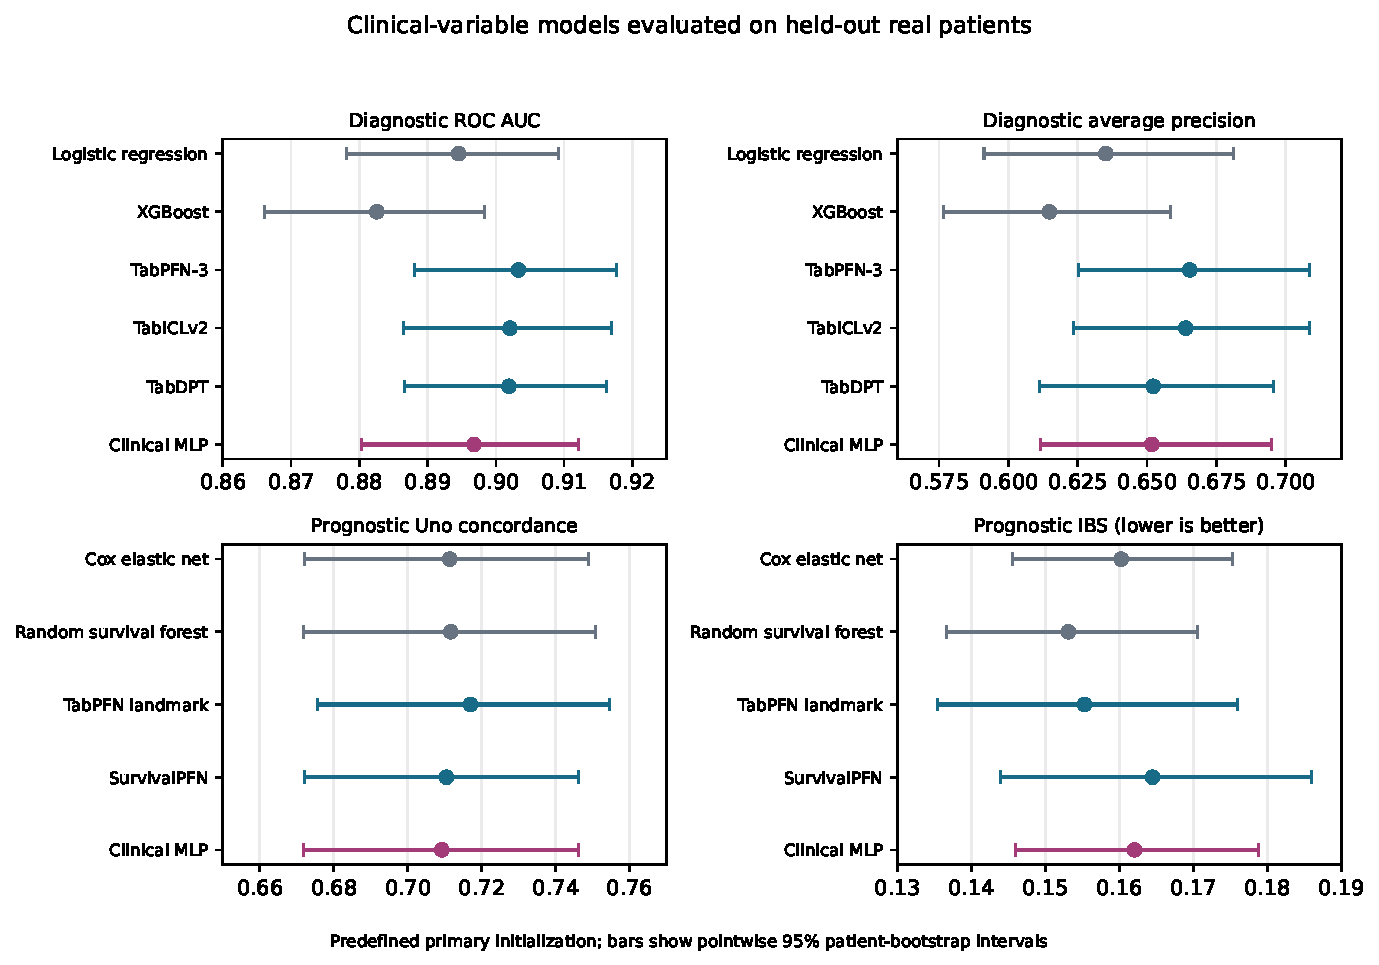
\includegraphics[width=0.94\linewidth]{mlp_heads/mlp_clinical_performance.pdf}
\caption{Clinical-variable performance on held-out real patients using the
predefined primary network initialization.  Points are estimates across the
matched evaluation partitions and bars are pointwise 95\% patient-bootstrap
intervals.  The clinical MLP is highlighted; lower IBS is favourable.}
\label{fig:mlp:clinical-performance}
\end{figure}

\begin{figure}[htbp]
\centering
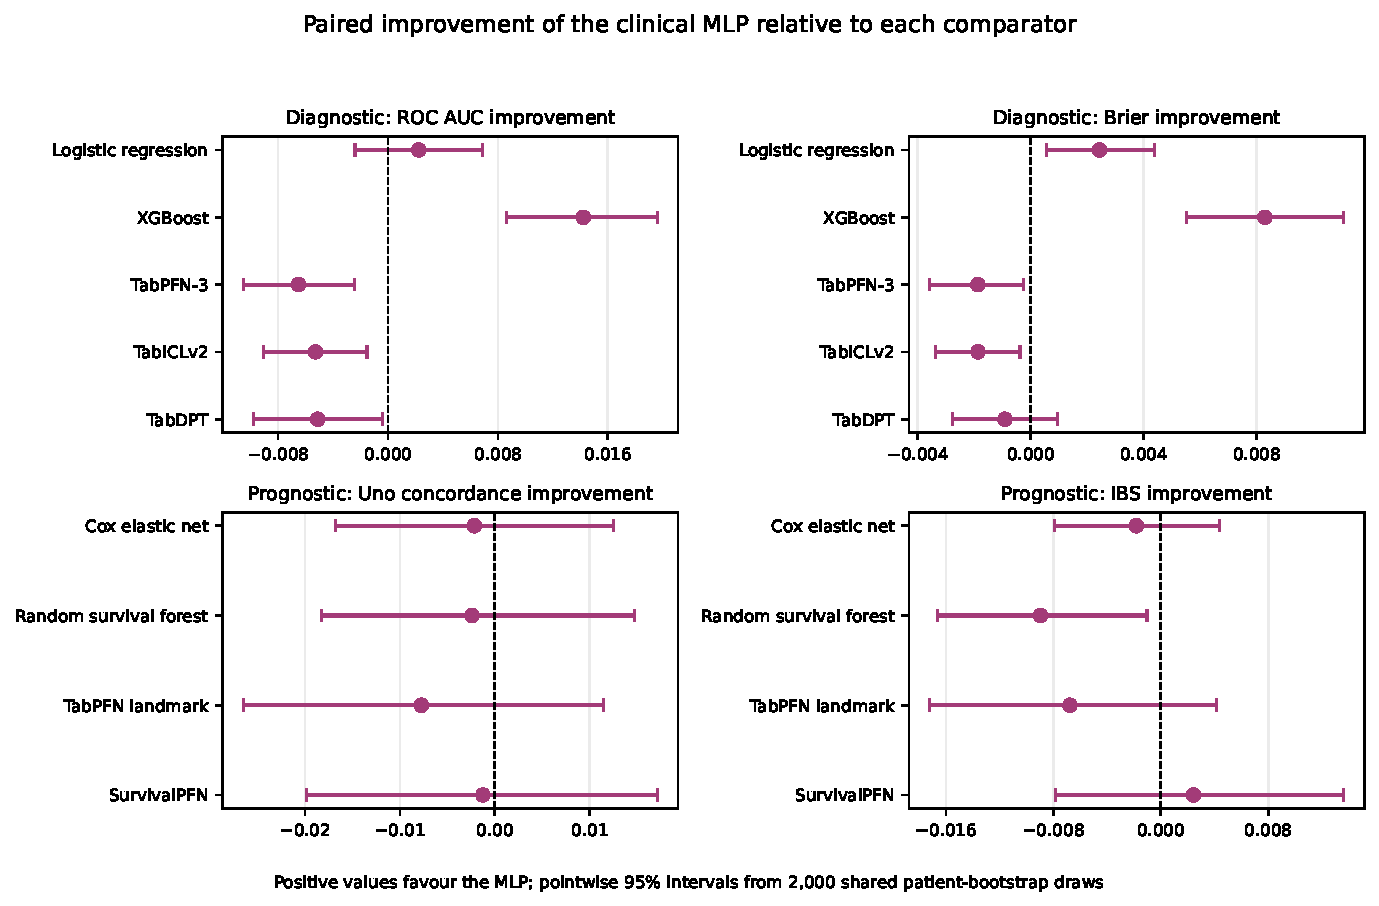
\includegraphics[width=0.94\linewidth]{mlp_heads/mlp_paired_improvements.pdf}
\caption{Paired improvement of the clinical MLP relative to each comparator.
Positive values favour the MLP in every panel.  The intervals use the same
2,000 patient resamples for both models and are not adjusted for the number of
comparisons.}
\label{fig:mlp:paired}
\end{figure}

\FloatBarrier
\subsection{Exploratory analysis of TabPFN representations}
\label{sec:mlp:embeddings}

For diagnosis, applying the MLP to the 512-dimensional TabPFN representation
produces essentially the same ROC AUC as regularized logistic regression: both
round to 0.897.  The paired ROC AUC difference is approximately zero, and the
intervals for average precision and Brier score also include zero
(Table~\ref{tab:mlp:embedding}).  For prognosis, the representation-based MLP
has lower point concordance and higher point IBS than the representation-based
Cox model, although both paired intervals narrowly include zero.  There is
therefore no consistent evidence that the nonlinear head extracts more useful
information from these representations than the corresponding linear heads.

\begin{table}[htbp]
\centering\footnotesize
\caption{Exploratory comparison of MLP and linear heads applied to the same
TabPFN representations.  Improvement is MLP minus linear head for
discrimination and linear head minus MLP for Brier score or IBS, so positive
values favour the MLP.  The representations were computed before the evaluation
partitions were formed.}
\label{tab:mlp:embedding}
\begin{tabularx}{\linewidth}{@{}p{1.55cm}p{2.1cm}rrY@{}}
\toprule
Task & Metric & MLP head & Linear head & Paired improvement [95\% interval] \\
\midrule
\csname @@input\endcsname{tables/mlp_heads/embedding_rows.tex}
\bottomrule
\end{tabularx}
\end{table}

These findings cannot be used to rank the clinical variables against the TabPFN
representations.  Although scaling is estimated within each training partition,
the underlying representations were already created using the full cohort.
The 2 input types also differ substantially in dimension: the representation
heads receive 512 or 1,024 inputs, whereas the clinical heads receive 31 or
26--27 encoded inputs.  The effects of representation, dimensionality and
optimization therefore cannot be separated in a direct comparison.

\subsection{Epoch selection, initialization variability and computation}
\label{sec:mlp:stability}

The selected training duration differs by task and input type
(Table~\ref{tab:mlp:robustness}).  The clinical diagnostic MLP selects a median
of 27 epochs, compared with 92 for clinical prognosis.  The representation
heads select medians of 7 and 13 epochs.  These differences do not show that one
input type learns a better predictor more quickly, because the input dimensions,
loss functions and validation-loss scales differ.  Every final network is
refitted for exactly its selected number of epochs.

\begin{table}[htbp]
\centering\scriptsize
\setlength{\tabcolsep}{3pt}
\caption{Epoch selection, variation across 3 network initializations and
observed computation time.  Epochs are shown as minimum/median/maximum.
Discrimination is ROC AUC for diagnosis and Uno concordance for prognosis;
probability error is Brier score and IBS, respectively.  Time is the median
fit-and-predict duration per evaluation partition for the primary initialization.}
\label{tab:mlp:robustness}
\begin{tabularx}{\linewidth}{@{}p{1.35cm}p{1.9cm}r p{1.55cm}YYr@{}}
\toprule
Task & Input & Selections & Epochs & Discrimination range & Error range & Time (s) \\
\midrule
\csname @@input\endcsname{tables/mlp_heads/robustness_rows.tex}
\bottomrule
\end{tabularx}
\end{table}

Diagnostic estimates change little across the 3 initializations: clinical ROC
AUC ranges from 0.8952 to 0.8968 and Brier score from 0.0878 to 0.0880.
Prognostic variation is larger but remains modest, with Uno concordance from
0.7026 to 0.7092 and IBS from 0.1621 to 0.1656.  The predefined primary
initialization gives the best clinical point estimate among these 3 runs for
the displayed metrics, but it was fixed before the results were examined.
Three initializations are not sufficient to characterize the complete range of
possible optimization outcomes.

\begin{figure}[htbp]
\centering
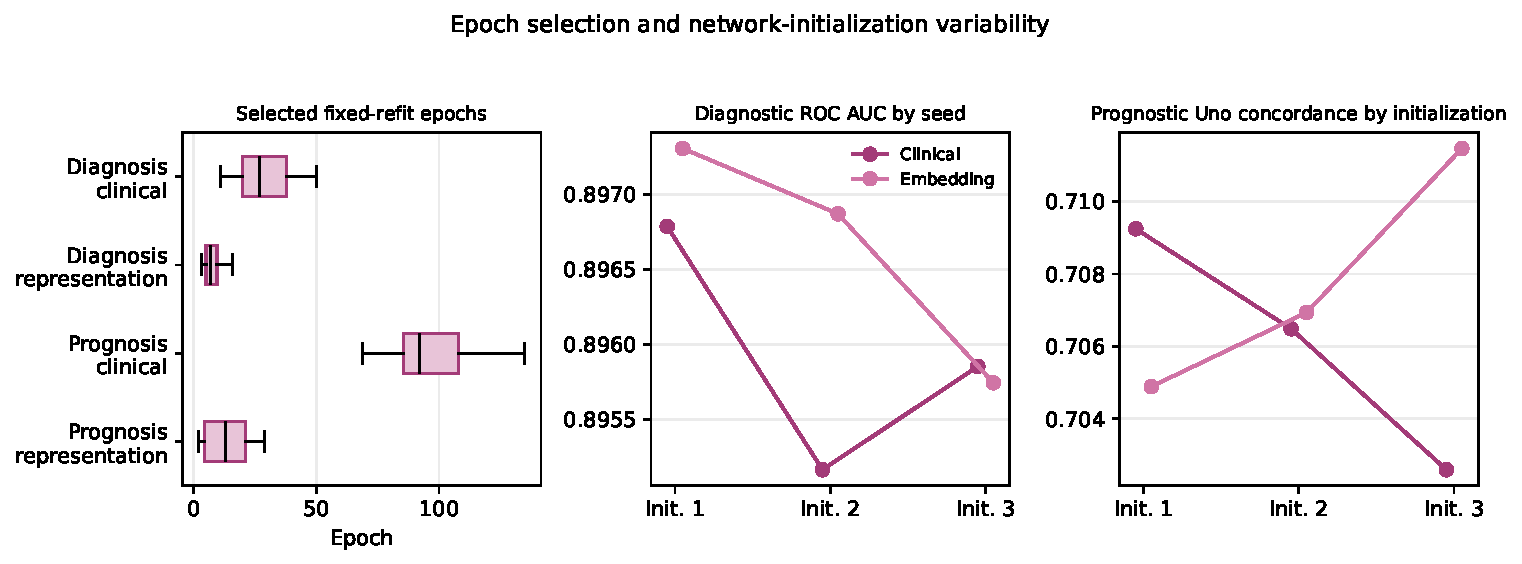
\includegraphics[width=0.96\linewidth]{mlp_heads/mlp_training_stability.pdf}
\caption{Selected epochs and variation across the 3 network initializations.
The left panel summarizes the selected epoch counts across evaluation
partitions.  The other panels show separate point estimates for each
initialization; connecting lines are visual guides and are not confidence
intervals or time trends.}
\label{fig:mlp:stability}
\end{figure}

\FloatBarrier
All networks were trained on the NVIDIA RTX 3060 Laptop graphics processing
unit (GPU) using NVIDIA's Compute Unified Device Architecture (CUDA).  Training
used 32-bit floating-point arithmetic and deterministic algorithms; the
lower-precision TensorFloat-32 mode was disabled.  The median fit-and-predict
time per evaluation partition was 1.44 seconds for clinical diagnosis and 0.64
seconds for clinical prognosis.  Maximum allocated GPU memory across the
real-patient MLP fits was approximately 70 MB.  These timings cover model
fitting and prediction on the study computer and should not be interpreted as
general hardware benchmarks.

\subsection{Interpretation and limitations}
\label{sec:mlp:limits}

The clinical MLP provides a direct test of whether a compact nonlinear model
improves on the preceding clinical-data benchmarks.  For diagnosis, it reduces
Brier score relative to logistic regression and performs better than XGBoost,
but it does not improve ROC AUC over logistic regression with clear statistical
support and remains below all 3 diagnostic TFMs on ROC AUC.  For prognosis, it
does not improve discrimination over any comparator and has worse IBS than the
RSF.  The exploratory representation analysis likewise finds no consistent
advantage over regularized logistic or Cox heads.  Nonlinearity alone therefore
does not explain the diagnostic advantage of the pretrained TFMs in this
cohort.

The conclusion is limited to one architecture and optimizer configuration; no
hyperparameter search was performed.  The bootstrap intervals hold the fitted
networks fixed, and 3 initializations provide only a partial view of optimization
variability.  Grade 4 is too rare for a reliable fold-level diagnostic conclusion
and does not meet the prognostic subgroup requirements in any split.  All
primary results are internal to one SEER extract, and these MLPs were not tested
in an independent clinical cohort.  The representation analysis is further
limited because the TabPFN transformation was computed before the evaluation
partitions were formed.  Overall, no general MLP advantage was demonstrated.
Section~\ref{sec:augmentation} next evaluates partition-specific augmentation.
